\documentclass[a4paper,10pt]{article}
\usepackage{graphicx} % Required for in\textit{SER}ting images
\usepackage[a4paper,top=2cm,bottom=2cm,left=3cm,right=3cm,marginparwidth=1.75cm]
{geometry}
\usepackage[colorinlistoftodos]{todonotes}
\usepackage[style=apa, backend=biber]{biblatex}
%\usepackage{geometry}
\DeclareLanguageMapping{english}{english-apa}
\addbibresource{literature.bib} % Link your .bib file here

\title{ICT3007: Management of Computer Engineering Projects\newline \centering Case Study 1 - Succession Transition and Company Turnaround}

\author{
Bahne J. Thiel-Peters (bthi0001)\\
Graham Pellegrini (gpel0001)
}

\begin{document}

\maketitle
\thispagestyle{empty}

\pagenumbering{arabic}
\setcounter{page}{1}

\section{Part C: Reflection}
\subsection{1.What did Julie decide to do about the leak of confidential information in Sam’s team? Discuss what she should have done? Why?}

What was done:
\begin{itemize}
    \item Julie decided to confront Sam directly about the leak of confidential information in his team.
    \item She decided not to escalate the issue to the board
    \item To avoid damaging Sams reputation and her own.
\end{itemize}

What should have been done and why:
\begin{itemize}
    \item Julie should have spoken to Sam in private about the leak of confidential information.
    \item She should have conviced and advised him to discuss this issue with Steve and John possibly at a board meeting.
    \item Since the leadership dynamic is small and still a family dynamic there shouldn't be reason to not discuss this issue with the board. 
    \item No ones reputation should be damaged if the issue is discussed in a professional mannerr.
\end{itemize}

\subsection{2. What did Sam decide to do about the software bug in Julie’s product? Discuss what he should have done? Why?}

What did Sam decide to do:
\begin{itemize}
    \item Sam decided to warn Julie directly
    \item He made sure to be sincere and respectful in his approach, making sure the situation was explained clearly.
    \item He would then later discuss the issue with the board, when the bug would be fixed and the time is right.
\end{itemize}

The group agreed with the actions taken by Sam. \\
By warning Julie directly, he made sure that she had the opportunity to fix the bug before it became a bigger issue. This act showed how Sam put the business first and is willing to work with Julie, showing good leadership skills.\\

He tries to enusre that Julie won't feel attacked by his confrontation, by being sincere and respectful. He then plans to discuss the issue with the board, when the bug is fixed and the time is right. This will shine light on both Julie for being able to handle the situation and fix the bug under pressure. As well as Sam for practicing the openess and transparency that he preached during the inital board meeting proposal.\\


\subsection{3. What did Steve decide to do about the conflict? Discuss what he should have done? Why?}

\subsubsection{What did Steve decide to do:}
Steve took 3 steps to mediate the conflict between Sam and Julie:

\begin{itemize}
    \item He facilitated a structured discussion to address the grievances of both parties.
    \item He allocated limited resources to Julie's RnD efforts to support her innovation while ensuring Sam's sales campaigns remain operational.
    \item He developed a balanced resource-sharing policy to clarify and enforce boundaries for office space, meeting rooms, and personnel allocation.
\end{itemize}

\subsubsection{What should have been done and why:}

While the steps taken by Steve were reasonable, he could have considerred taking some additional steps to address the root cause of the conflict with more effect.\\
\begin{itemize}
    \item Establish Clear Role Definitions from the Outset, in order to clearly define Sam and Julie's boundaries of authority and responsibility.
    \item Create a Joint Planning Framework, so that Sam and Julie can work together to develop a shared vision and strategy for the company.
    \item Address the Underlying Cultural Issue, there might have been competitive pressures, team building activities and meetings could have been used to address this.
\end{itemize}

These steps are important to include as they help to prevent the issue from happening again, rather than simply solving it when it cropped up.

\subsection{4. What did John decide to do about monitoring Sam and Julie? Discuss what he should have done? Why?}

\subsubsection{What did John decide to do:}
John implemented several measures to monitor Sam and Julie's progress and performance:

\begin{itemize}
    \item He evaluated their performance using quantitative metrics such as sales growth, market penetration, and timely delivery of new products.
    \item He collected qualitative feedback through periodic one-on-one sessions with Sam and Julie, as well as by observing their interactions during board meetings.
    \item He occasionally gathered team feedback to assess their leadership styles and the morale of their respective divisions.
    \item He reviewed quarterly divisional reports to ensure both leaders were meeting their set goals and expectations.
\end{itemize}

\subsubsection{What should have been done and why:}
Although John's measures were a step in the right direction, a more comprehensive and proactive approach to monitoring could have been implemented to address leadership and team challenges more effectively. This could have included the following:

\begin{itemize}
    \item \textbf{Establish Regular Employee Surveys:} Conducting anonymous surveys to monitor team morale, workload, and satisfaction on a regular basis. This would provide insights into potential burnout and dissatisfaction before they escalate.
    \item \textbf{Introduce Real-Time Feedback Mechanisms:} Encouraging open communication between Sam, Julie, and their teams, creating a culture where feedback is provided and acted upon continuously.
    \item \textbf{Define Key Leadership KPIs:} Setting clear, measurable leadership KPIs focused not only on divisional performance but also on employee retention, team satisfaction, and leadership effectiveness.
    \item \textbf{Provide Mentorship and Leadership Training:} Establishing regular mentorship sessions for Sam and Julie to address their leadership gaps—helping Sam become more decisive and Julie more inclusive.
    \item \textbf{Monitor Workload and Resource Allocation:} Regularly reviewing team workloads to ensure equitable distribution and prevent burnout, ensuring teams are not stretched beyond their capacity.
\end{itemize}


\section{Post Announcement}
\subsection{5. Discuss the consequences of the announcement}
The announcement stated that John had created a fake scenario to test Sam and Julie.\\

\textbf{Positive Consequences:}
\begin{itemize}
    \item Through the announcement, Sam and Julie now know how each other would react in similar situations.
    \item This might bring them to trust each other further.
    \item John gained the reassurance that Sam and Julie are capable of working together and handling difficult situations.
\end{itemize}

\textbf{Negative Consequences:}
\begin{itemize}
    \item The announcement makes John seem unreliable, not respecting the family values that he preeched and enforced.
    \item Although it might have been intended for good reasons, it envoked a disturbing scene that they had to tackle during operation.
    \item Steve will see this action from John as unprofessional. There would have been other ways to test their leadership principles, without going behind their back and causing drama.
    \item Steve might be taken a back from Jonh's actions and might reconsider his position in the company.
    \item The announcement caused a rift between the family members, which is not desirable in a family business.
    \item An enviroment of uncertainty has been created, which puts other on edge.
    \item This issue could trickle down to the employees, causing them to feel uncertain about the company's future and the people managing it.
\end{itemize}

\subsection{6. Motivating the staff}

\begin{itemize}
    \item Revise the company’s mission and vision statements to inspire and re-align the team with organizational goals.
    \item Implement effective workload management to better distribute and schedule tasks, reducing burnout.
    \item Establish a \textit{talent development team} to engage employees in proposing innovative product ideas.
    \item Organize \textit{team-building activities}, such as dinners, sports events, and other social engagements, to foster camaraderie.
    \item Enhance the \textit{feedback system} by introducing 360-degree feedback to provide comprehensive and constructive performance insights.
    \item Increase communication through frequent check-ins with employees to address concerns and improve morale.
    \item Adopt a \textit{democratic leadership style} to ensure employees feel heard and valued within the organization.
    \item Encourage Julie to delegate important tasks to her team, promoting involvement and ownership in the decision-making process.
\end{itemize}

\textbf{Why care about retaining the staff?}\newline
Sam and Julie should prioritize retaining their staff to ensure continuity, maintain productivity, and avoid the high costs of recruitment and training. Experienced employees hold valuable knowledge that drives innovation and sustains growth, while frequent turnover disrupts morale and team efficiency. Retaining motivated staff fosters a positive reputation, attracts talent, and supports long-term success by keeping the company competitive and aligned with strategic goals.

\subsection{7. Role Changes and Responsibilities}

The company faces a critical decision regarding its future leadership structure. Three potential scenarios are being considered, each with its own implications. Below, the advantages and disadvantages of each option are explored in detail.

\subsubsection*{Option 1: Maintaining the Current Roles and Responsibilities}

\subsubsection*{Advantages}
This approach ensures continuity, which can be valuable if the company is already performing well. The existing structure avoids disruption, as there would be no need to retrain or hire new personnel. Furthermore, the current organizational framework would remain intact, simplifying operations.

\subsubsection*{Disadvantages}
While maintaining the status quo provides stability, it may not address the ambitions of Sam and Julie, who are eager for greater responsibilities. Additionally, Steve’s prolonged role as CEO could lead to discomfort among family members, as he continues to wield significant influence. Steve may also be nearing retirement, and the absence of a transition plan could leave the company unprepared for his eventual departure.

\subsubsection*{Option 2: Transitioning Steve to a Non-Executive Director Role, with Sam as CEO and Julie as CTO}

\subsubsection*{Advantages}
This structure allows Steve to step back from daily operations while continuing to provide guidance as a non-executive director. Both Sam and Julie would have the opportunity to take on larger roles, aligning with their ambitions. Sam’s leadership skills could be more effectively utilized in the CEO role, while Julie’s technical expertise would thrive in the CTO position. Steve’s mentoring role ensures continuity, and Julie could still contribute to technical strategy while Sam gains the confidence and experience needed to make final decisions.

\subsubsection*{Disadvantages}
There is a risk that Julie may feel overlooked if she aspires to the CEO position, which could impact her satisfaction and motivation. Additionally, Steve might find it difficult to fully let go of operational control, which could create tension during the transition. Lastly, while Sam has shown leadership potential, he may still lack the experience needed to handle the full scope of the CEO responsibilities.

\subsubsection*{Option 3: Joint Leadership by Sam and Julie as Co-CEOs, with Steve Retiring}

\subsubsection*{Advantages}
This option allows Sam and Julie to share decision-making responsibilities, leveraging their combined strengths to lead the company effectively. By working together, they can learn from one another, balancing Sam’s leadership style with Julie’s technical expertise. Additionally, Steve’s retirement would give him the opportunity to enjoy personal time while ensuring the family maintains control of the company.

\subsubsection*{Disadvantages}
Shared leadership poses risks, as disagreements between Sam and Julie could delay decision-making and affect the company’s efficiency. There is also a chance that their working relationship could become strained under the pressures of joint leadership. Furthermore, Steve may struggle to completely detach from the company, potentially complicating the transition.

\subsubsection*{Decision and Justification}

After evaluating all options, the second option is determined to be the most suitable. This approach strikes a balance between progression and stability. Steve’s transition to a non-executive director role ensures his experience and guidance remain available. Sam’s appointment as CEO allows him to refine his leadership skills, while Julie’s new role as CTO leverages her technical expertise to drive innovation. This structure also fosters collaboration, as Julie continues to support Sam in technical strategy while he gains confidence in his decision-making. Overall, this arrangement prepares the company for sustainable growth while maintaining alignment with family values.


\section{References}

\pagebreak
\begin{figure}[h]
    \centering
    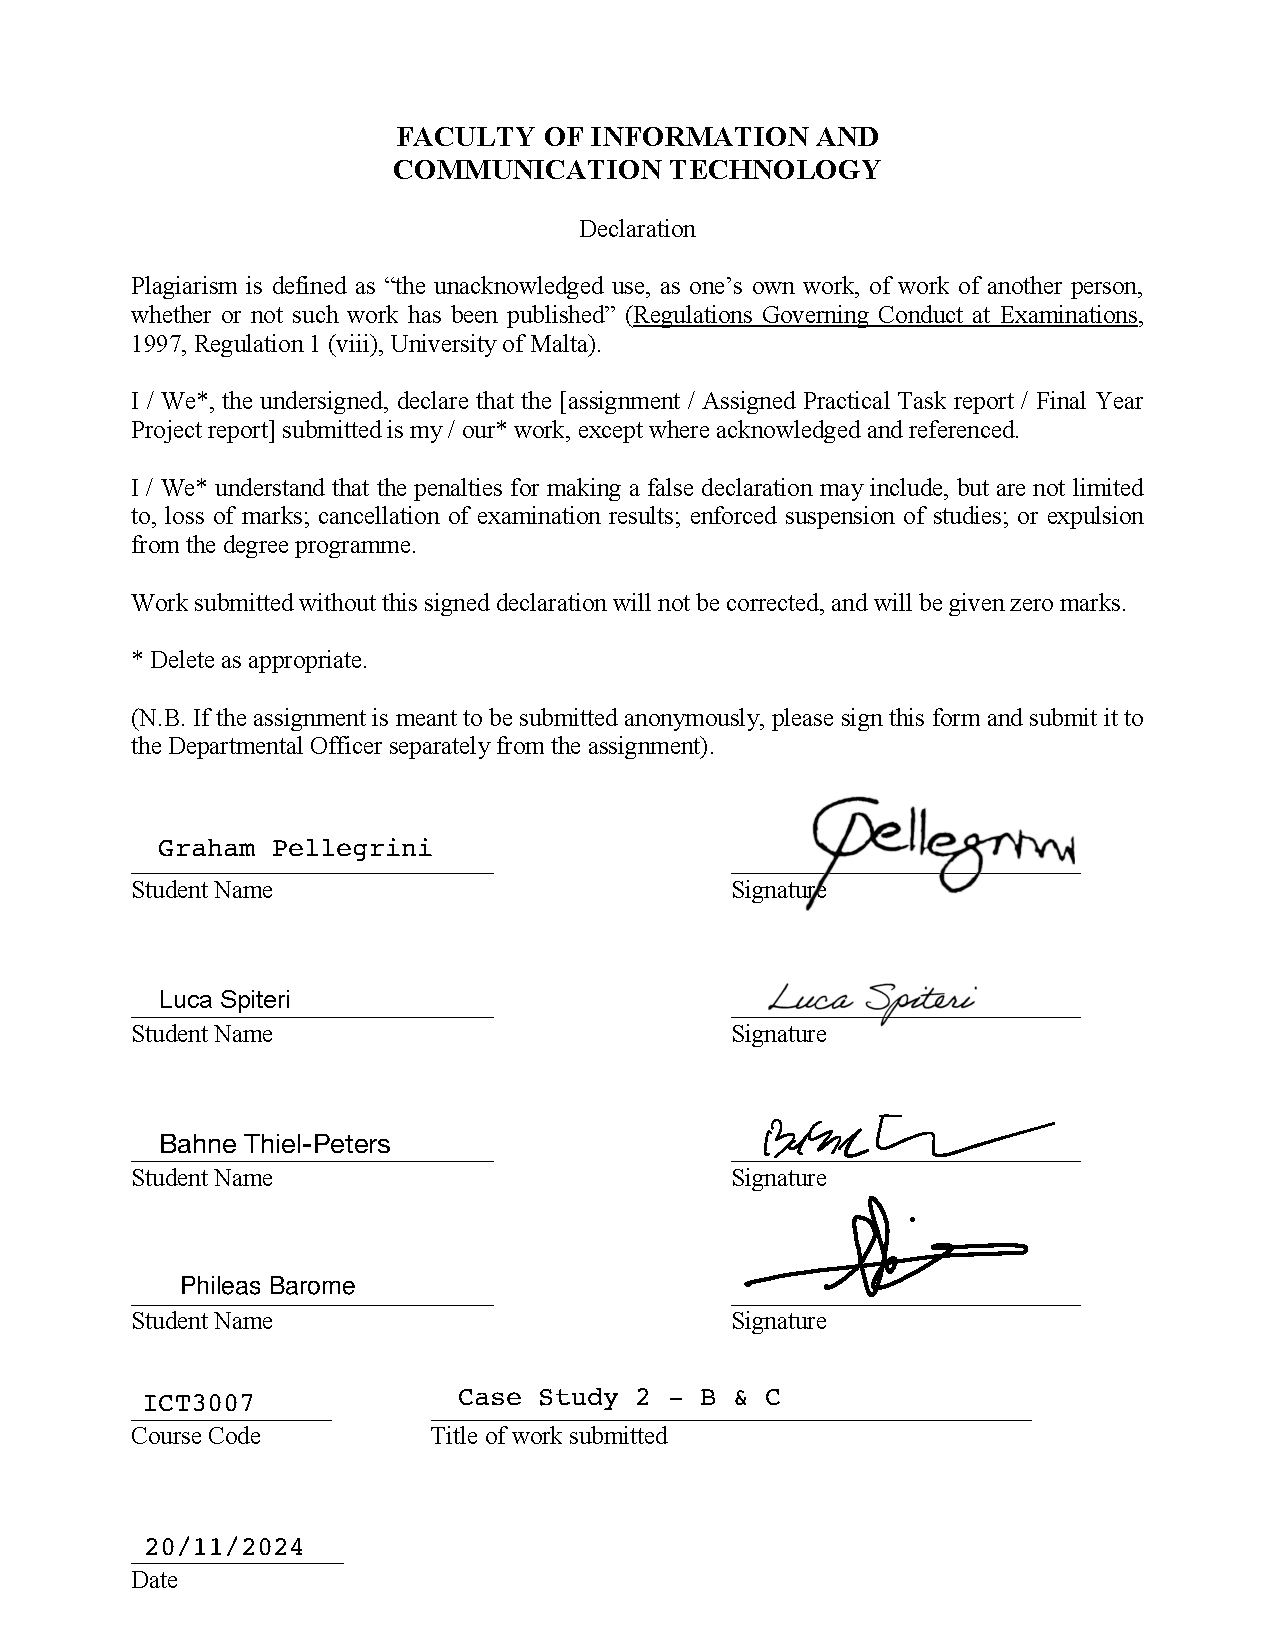
\includegraphics[width=1\textwidth]{Group_Plagiarism_Form.pdf}
    \caption{Group Plagiarism Form}
\end{figure}
\end{document}
